\documentclass[11pt, a4paper]{article}

% --- Packages (template set, plus url/tikz/amsmath for figures and formulae) ---
\usepackage[utf8]{inputenc}
\usepackage[T1]{fontenc}
\usepackage{mathptmx} % Times New Roman font for professional document typography
\usepackage{graphicx}
\usepackage[margin=0.8in]{geometry}
\usepackage{xcolor}
\usepackage{titlesec}
\usepackage{enumitem}
\usepackage{float}
\usepackage{booktabs}
\usepackage{multirow}
\usepackage{array}
\usepackage{amsmath}
\usepackage{url}
% Let long paths and module names break at . / _ - so they never run into the margin.
\def\UrlBreaks{\do\.\do\/\do\_\do\-\do\{\do\}\do\|}
\def\UrlBigBreaks{}
\newcolumntype{L}[1]{>{\raggedright\arraybackslash}p{#1}}
% A line holding only an unbreakable URL may stretch rather than overflow the margin.
\setlength{\emergencystretch}{3em}
\usepackage{tikz}
\usetikzlibrary{positioning, arrows.meta, fit, calc}

% --- Amrita Colors ---
\definecolor{amritaMaroon}{HTML}{A4123F}
\definecolor{tierFill}{HTML}{FBEFF3}
\definecolor{dataFill}{HTML}{EEF6F5}
\definecolor{offFill}{HTML}{FDF7EC}

% --- Title & Section Formatting ---
\titlespacing*{\section}{0pt}{12pt}{4pt}
\titlespacing*{\subsection}{0pt}{8pt}{3pt}
\titleformat{\section}{\large\bfseries\color{amritaMaroon}}{\thesection}{0.8em}{}
\titleformat{\subsection}{\normalsize\bfseries\color{amritaMaroon}}{\thesubsection}{0.6em}{}

\pagestyle{plain}

% Anything only the team can supply is printed in red so it cannot slip through.
\newcommand{\fillin}[1]{\textcolor{red}{\textbf{[#1]}}}

% Movies & TV, LightGCN ranked by dot product (local rerun) - filled from
% reports/benchmarks/movies_and_tv_lightgcn_dot_local.json
\newcommand{\mvDotR}{\textbf{0.0454}}
\newcommand{\mvDotN}{\textbf{0.0194}}
\newcommand{\mvDotM}{\textbf{0.0121}}

\begin{document}

% ==========================================
% HEADER & TITLE BLOCK
% ==========================================
\noindent
\begin{minipage}{\textwidth}
    \centering
    {\Large \textbf{\textcolor{amritaMaroon}{
    AMRITA VISHWA VIDYAPEETHAM \\
    SCHOOL OF COMPUTING \\
    DEPARTMENT OF COMPUTER SCIENCE AND ENGINEERING \\
    }}}
    \vspace{0.2cm}
    {\large \textbf{Real-Time Adaptive Cross-Media Recommendation System:\\ A Domain-Agnostic Engine with Audience Eligibility}} \\[0.1cm]
    \textbf{23CSE498 -- Project Phase II (External Review)} \quad | \quad \textbf{Team Number: G022} \\
    \today
\end{minipage}

\vspace{0.3cm}
\hrule
\vspace{0.3cm}

% --- Team & Guide Details ---
\noindent
\begin{center}
    \renewcommand{\arraystretch}{1.45}
    \setlength{\tabcolsep}{6pt}
    \begin{tabular}{|l|p{4.4cm}|p{4.6cm}|p{3.0cm}|}
        \hline
        \multicolumn{2}{|c|}{\textbf{Team Members}} & \textbf{Project Guides} & \textbf{Project Type} \\
        \hline
        \small CB.SC.U4CSE23051 & \small \raggedright Sanjay A. K. &
        \multirow{4}{=}{\raggedright \small \textbf{Dr. Bagavathi Sivakumar P.} \newline \textit{\fillin{Designation}, Dept. of CSE} \newline \textbf{Dr. Krishna Priya G.} \newline \textit{\fillin{Designation}, Dept. of CSE}} &
        \multirow{4}{=}{\raggedright \small \textbf{Type 3} \newline Software-Based Project} \\ \cline{1-2}
        \small CB.SC.U4CSE23022 & \small Eswara Raj M. & & \\ \cline{1-2}
        \small CB.SC.U4CSE23324 & \small Aditya Vijay & & \\ \cline{1-2}
        \small CB.SC.U4CSE23359 & \small Himaneesh Reddy Jangalapalli & & \\
        \hline
    \end{tabular}
\end{center}
\vspace{0.2cm}

\section{Abstract}
\noindent
Recommendation systems are usually built for one kind of item, and they usually apply age or safety rules \emph{after} ranking, where a reranker can promote an ineligible item back onto the page. This project delivers a domain-agnostic recommendation engine over 120,747 items in seven content types (movies, shows, books, music, health, industrial and finance products). A user describes what they want in free text. The engine retrieves candidates by meaning (Sentence-BERT embeddings in a Qdrant vector store) and by exact creator and title matching, removes everything the viewer may not see (age, safe mode, domain, risk tier) \emph{inside} the vector query, and reranks the survivors with a LightGCN collaborative signal, a live exponential-moving-average (EMA) taste vector and profile signals. Every like, skip or rating updates the next search immediately, with no retraining. The system is a three-tier web application: a React 19 single-page client, a FastAPI service with 16 endpoints including email and Google accounts, and MySQL 8 plus Qdrant for persistence. It is fully integrated and runs end to end with one command. Verification covers 381 automated tests (unit, integration, regression), a live latency study (p95 455 ms), an audience-constraint evaluation with zero eligibility violations, and offline ranking benchmarks on Amazon Reviews 2023, including the Neural Collaborative Filtering baseline requested at the previous review. The research results were accepted at ICMLDE 2026 \cite{ak2026crossmedia}.

% --- 2. SOFTWARE REQUIREMENTS SPECIFICATION (SRS) ---
\section{Software Requirements Specification (SRS)}

\subsection{Product Scope, Actors \& Use Cases}
\begin{itemize}[noitemsep, topsep=2pt]
    \item \textbf{Software Purpose \& Scope:} One recommendation engine that serves entertainment, health, industrial and finance catalogues through the same retrieval and ranking stack, where a new vertical is a configuration entry (\texttt{config/domains.yaml}) rather than new code. Health and finance are scoped to \emph{information and product discovery}: the system gives no medical, diagnostic or investment advice, attaches an advisory to those domains, and withholds high-risk items by default.
    \item \textbf{User Roles / Actors:} (i)~\emph{Visitor}, who explores through one of 13 seeded demo personas without an account; (ii)~\emph{Registered user}, signed in with email and password or Google, whose interactions personalise their own results; (iii)~\emph{Guardian / safe-mode viewer}, for whom results are capped at a child ceiling; (iv)~\emph{Data engineer}, who runs the offline pipeline (fetch, catalogue build, embeddings, vector index, model training); (v)~\emph{External services}: TMDb \cite{tmdb}, Open Library \cite{openlibrary}, Last.fm \cite{lastfm}, Amazon Reviews 2023 \cite{hou2024amazon} and Google Identity.
    \item \textbf{Comparison with Existing Systems:} Most recommenders serve a single domain, and cross-domain methods usually transfer between two domains \cite{zang2022cross,zhang2025survey}. Collaborative filtering such as LightGCN \cite{he2020lightgcn} needs interaction history and cannot serve a new user. Pure vector search answers intent well but misses titles with no semantic content (a vector search for ``F1'' returned a song while the film was in the catalogue). Age filtering applied after ranking can leak ineligible items. This system combines semantic, lexical and collaborative evidence, and enforces eligibility before any item is scored.
    \item \textbf{Core Use Cases:}
    \begin{enumerate}[noitemsep, topsep=2pt]
        \item \textbf{Search and recommend.} Actor: visitor or user. Pre: catalogue and index loaded. Flow: type a query $\rightarrow$ typo correction $\rightarrow$ creator, title and semantic retrieval under the eligibility filter $\rightarrow$ rerank $\rightarrow$ result cards with a per-signal score breakdown. Post: ranked, eligible results with an advisory for regulated domains.
        \item \textbf{Give feedback and adapt.} Actor: user. Pre: results shown. Flow: like, save, skip, mark done or rate $\rightarrow$ event logged $\rightarrow$ EMA taste vector updated in the same request. Post: the next search reflects the feedback; a second click on a toggle undoes it.
        \item \textbf{Audience-safe browsing.} Actor: guardian. Flow: switch on safe mode or declare an age $\rightarrow$ the ceiling is compiled into the vector query. Post: no item above the ceiling is retrieved; an undeclared viewer is capped at the teen ceiling (fail-closed).
        \item \textbf{Account lifecycle.} Actor: new user. Flow: sign up $\rightarrow$ pick starter items (one per genre) $\rightarrow$ personalised search $\rightarrow$ optional self-service deletion of the account and all its data. Post: deletion removes interactions, profile, sessions and the user row in one transaction.
    \end{enumerate}
\end{itemize}

\subsection{Functional \& Non-Functional Requirements}
\begin{table}[H]
    \centering
    \footnotesize
    \renewcommand{\arraystretch}{1.25}
    \begin{tabular}{|c|L{3.0cm}|L{9.9cm}|}
        \hline
        \textbf{Req. ID} & \textbf{Category} & \textbf{Requirement Specification} \\
        \hline
        FR-01 & Functional & Free-text hybrid retrieval over all domains: creator and title matching plus Sentence-BERT semantic search, with typo correction and autocomplete. \\
        \hline
        FR-02 & Functional & Audience eligibility (age, safe mode, domain, risk tier) enforced inside retrieval, so no ineligible item is ever scored or shown. \\
        \hline
        FR-03 & Functional & Real-time personalisation: each interaction updates the user's taste vector immediately; collaborative (LightGCN) and profile signals rerank results. \\
        \hline
        FR-04 & Functional & Explainability: each result shows how many points every signal contributed, and what changes if a signal is removed. \\
        \hline
        FR-05 & Functional & Accounts: email and Google sign-in, onboarding picks, per-account data access, and self-service account deletion. \\
        \hline
        NFR-01 & Performance & A recommendation request completes in under 500 ms at the 95th percentile on a single machine (measured: 455 ms). \\
        \hline
        NFR-02 & Security & Argon2id password hashes; random session tokens stored only as SHA-256 hashes in an HttpOnly cookie; login lockout after five wrong passwords that survives a restart; an account's data needs that account's session (401/403). \\
        \hline
        NFR-03 & Safety \& integrity & Every unknown fails closed (no age $\rightarrow$ teen ceiling; unknown label $\rightarrow$ most restrictive); an internal error is never answered with an unfiltered search. \\
        \hline
        NFR-04 & Maintainability & Domains and maturity rules are configuration; the full test suite runs without data or services and on every push (CI). \\
        \hline
    \end{tabular}
    \caption{Software Functional and Non-Functional Requirements Specification}
\end{table}

% --- 3. SOFTWARE ARCHITECTURE & SYSTEM DESIGN ---
\section{Software Architecture \& System Design}

\subsection{High-Level System Architecture}
\noindent
The system is a layered three-tier application with a separate offline pipeline (Fig.~\ref{fig:arch}). The \textbf{client tier} is a React single-page application that talks to the server only through a JSON API. The \textbf{service tier} is a FastAPI application; heavy objects (the SBERT encoder, the catalogue lookup tables and the Qdrant client) are created once at startup and injected into handlers. A request passes two stages: \emph{eligibility}, which compiles the viewer's constraints into a Qdrant filter, then \emph{relevance}, which fuses the signals additively. The \textbf{data tier} holds the vector index (Qdrant, $120{,}747 \times 384$), the relational store (MySQL 8: catalogue mirror, interaction log, profiles and accounts) and model artefacts. The \textbf{offline pipeline} builds the catalogue from public sources, encodes it, loads the index and the database, and trains the collaborative models.

\begin{figure}[H]
\centering
\resizebox{\textwidth}{!}{%
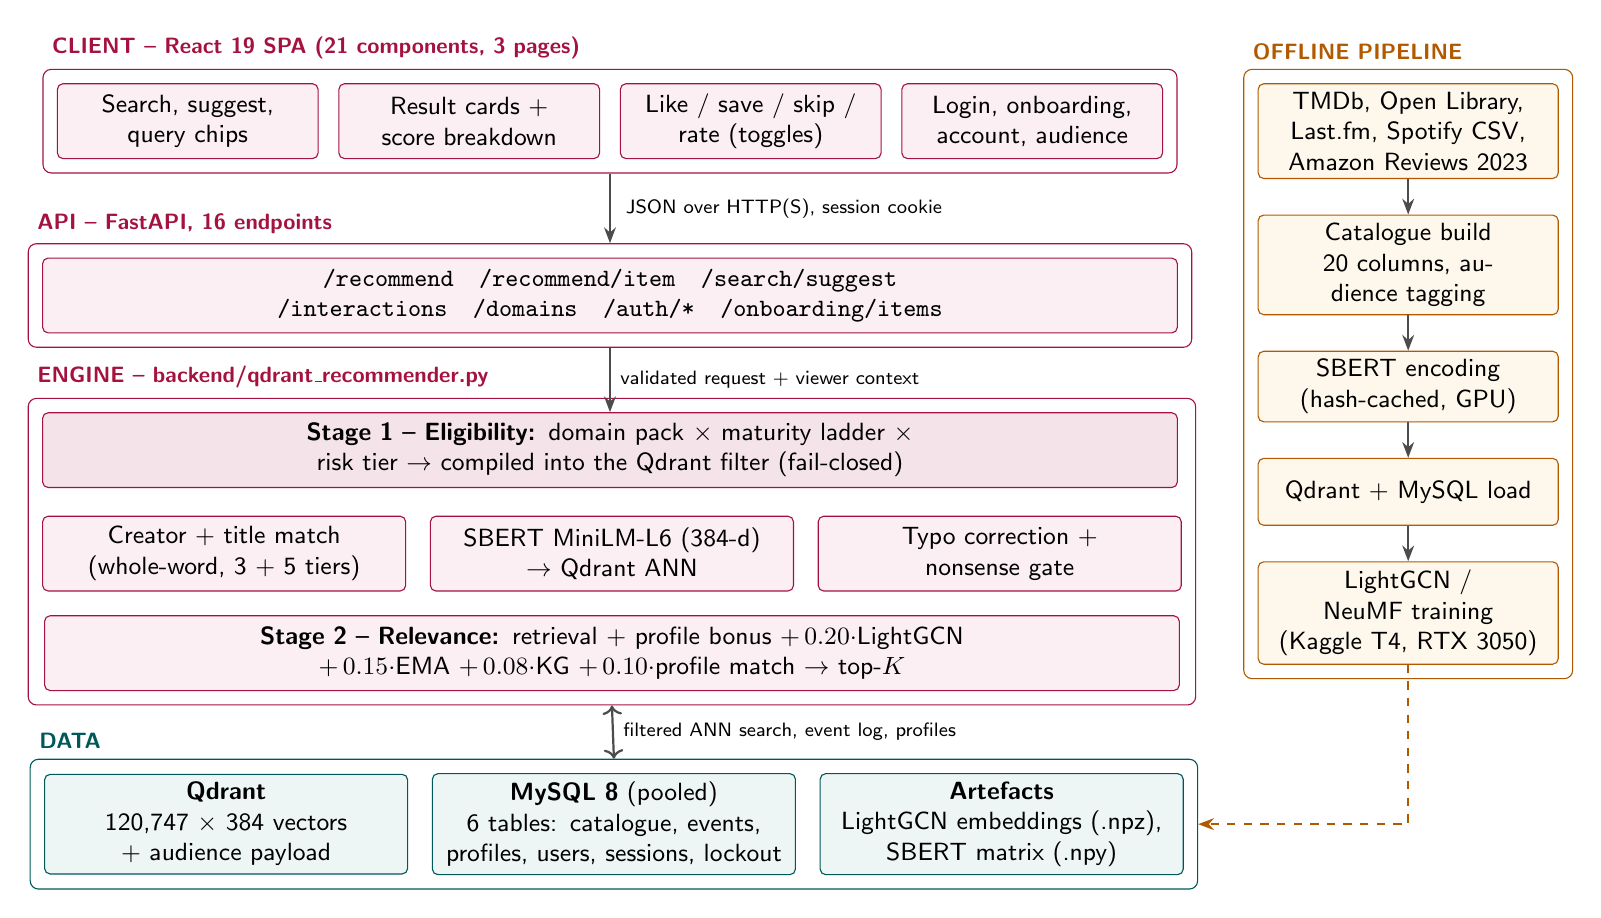
\begin{tikzpicture}[
    font=\sffamily\small,
    box/.style={draw=amritaMaroon, fill=tierFill, rounded corners=2pt, align=center, minimum height=0.95cm, inner sep=3pt},
    dbox/.style={draw=teal!70!black, fill=dataFill, rounded corners=2pt, align=center, minimum height=0.95cm, inner sep=3pt},
    obox/.style={draw=orange!70!black, fill=offFill, rounded corners=2pt, align=center, minimum height=0.85cm, text width=3.6cm, inner sep=3pt},
    tier/.style={draw=amritaMaroon, rounded corners=3pt, inner sep=5pt},
    lbl/.style={font=\sffamily\bfseries\footnotesize, text=amritaMaroon},
    arr/.style={-{Stealth[length=2mm]}, thick, draw=black!70}
]
% Client tier
\node[box, text width=3.1cm] (c1) {Search, suggest,\\ query chips};
\node[box, text width=3.1cm, right=0.25cm of c1] (c2) {Result cards +\\ score breakdown};
\node[box, text width=3.1cm, right=0.25cm of c2] (c3) {Like / save / skip /\\ rate (toggles)};
\node[box, text width=3.1cm, right=0.25cm of c3] (c4) {Login, onboarding,\\ account, audience};
\node[tier, fit=(c1)(c4), label={[lbl, anchor=south west]north west:CLIENT \textendash{} React 19 SPA (21 components, 3 pages)}] (client) {};

% API tier
\node[box, text width=14.2cm, below=1.25cm of $(c2.south)!0.5!(c3.south)$] (api) {\texttt{/recommend}\quad \texttt{/recommend/item}\quad \texttt{/search/suggest}\quad \texttt{/interactions}\quad \texttt{/domains}\quad \texttt{/auth/*}\quad \texttt{/onboarding/items}};
\node[tier, fit=(api), label={[lbl, anchor=south west]north west:API \textendash{} FastAPI, 16 endpoints}] (apit) {};

% Engine
\node[box, text width=14.2cm, below=1.0cm of api, fill=amritaMaroon!12] (gate) {\textbf{Stage 1 \textendash{} Eligibility:} domain pack $\times$ maturity ladder $\times$ risk tier $\rightarrow$ compiled into the Qdrant filter (fail-closed)};
\node[box, text width=4.4cm, below=0.35cm of gate.south west, anchor=north west] (r1) {Creator + title match\\ (whole-word, 3 + 5 tiers)};
\node[box, text width=4.4cm, right=0.3cm of r1] (r2) {SBERT MiniLM-L6 (384-d)\\ $\rightarrow$ Qdrant ANN};
\node[box, text width=4.4cm, right=0.3cm of r2] (r3) {Typo correction +\\ nonsense gate};
\node[box, text width=14.2cm, below=0.3cm of r2.south, anchor=north, xshift=0cm] (fuse) {\textbf{Stage 2 \textendash{} Relevance:} retrieval $+$ profile bonus $+\,0.20\cdot$LightGCN $+\,0.15\cdot$EMA $+\,0.08\cdot$KG $+\,0.10\cdot$profile match $\rightarrow$ top-$K$};
\node[tier, fit=(gate)(r1)(r3)(fuse), label={[lbl, anchor=south west]north west:ENGINE \textendash{} backend/qdrant\_recommender.py}] (eng) {};

% Data tier
\node[dbox, text width=4.4cm, below=1.05cm of fuse.south west, anchor=north west] (d1) {\textbf{Qdrant}\\ 120,747 $\times$ 384 vectors\\ + audience payload};
\node[dbox, text width=4.4cm, right=0.3cm of d1] (d2) {\textbf{MySQL 8} (pooled)\\ 6 tables: catalogue, events,\\ profiles, users, sessions, lockout};
\node[dbox, text width=4.4cm, right=0.3cm of d2] (d3) {\textbf{Artefacts}\\ LightGCN embeddings (.npz),\\ SBERT matrix (.npy)};
\node[tier, draw=teal!70!black, fit=(d1)(d3), label={[lbl, text=teal!70!black, anchor=south west]north west:DATA}] (data) {};

% Offline pipeline
\node[obox, right=1.2cm of c4.north east, anchor=north west] (o1) {TMDb, Open Library,\\ Last.fm, Spotify CSV,\\ Amazon Reviews 2023};
\node[obox, below=0.45cm of o1] (o2) {Catalogue build\\ 20 columns, audience tagging};
\node[obox, below=0.45cm of o2] (o3) {SBERT encoding\\ (hash-cached, GPU)};
\node[obox, below=0.45cm of o3] (o4) {Qdrant + MySQL load};
\node[obox, below=0.45cm of o4] (o5) {LightGCN / NeuMF training\\ (Kaggle T4, RTX 3050)};
\node[tier, draw=orange!70!black, fit=(o1)(o5), label={[lbl, text=orange!70!black, anchor=south west]north west:OFFLINE PIPELINE}] (off) {};

\draw[arr] (client.south) -- node[right, font=\sffamily\scriptsize, xshift=2pt]{JSON over HTTP(S), session cookie} (apit.north);
\draw[arr] (apit.south) -- node[right, font=\sffamily\scriptsize]{validated request + viewer context} (gate.north);
\draw[arr, <->] (eng.south) -- node[right, font=\sffamily\scriptsize]{filtered ANN search, event log, profiles} (data.north);
\draw[arr] (o1) -- (o2); \draw[arr] (o2) -- (o3); \draw[arr] (o3) -- (o4); \draw[arr] (o4) -- (o5);
\draw[arr, dashed, draw=orange!70!black] (o5.south) |- (data.east);
\end{tikzpicture}}
\caption{High-Level Software System Architecture (request path on the left, offline pipeline on the right; the dashed edge is the trained artefact that crosses into serving).}
\label{fig:arch}
\end{figure}

\subsection{Database Schema \& Data Modeling}
\noindent
MySQL holds six tables (Fig.~\ref{fig:er}). \texttt{content\_entities} mirrors the catalogue with a case-sensitive \path{global_id} key (\path{type:source:id}). \texttt{user\_interactions} is an append-only event log indexed on \path{(user_id, timestamp)}, with a foreign key to the catalogue that cascades on delete. \texttt{user\_profiles} stores declared preferences and the 384-d EMA taste vector as JSON. Accounts live in \texttt{users} (unique email and Google subject) and \texttt{user\_sessions} (only the SHA-256 of each session token; cascades with the user). \texttt{login\_failures} records wrong passwords so a lockout survives a restart. The audience fields (domain, maturity, minimum age, risk tier) are stored as integers in the Qdrant payload, where the eligibility filter is evaluated. Schema creation and migrations are idempotent, and connections come from a shared pool of ten.

\begin{figure}[H]
\centering
\resizebox{0.98\textwidth}{!}{%
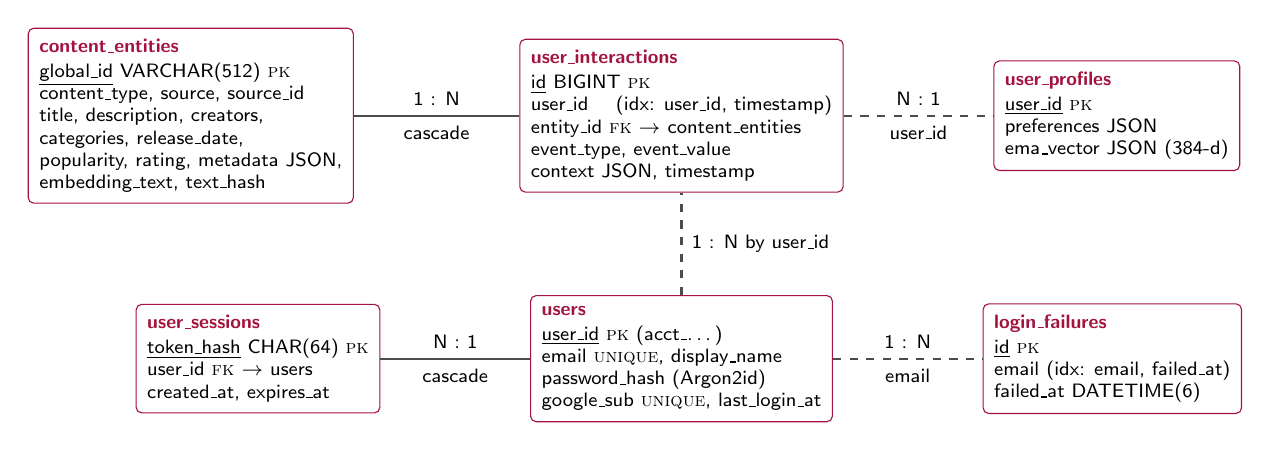
\begin{tikzpicture}[
    font=\sffamily\scriptsize,
    ent/.style={draw=amritaMaroon, rounded corners=2pt, align=left, inner sep=4pt, fill=white},
    rel/.style={thick, draw=black!70},
]
\node[ent] (ce) {\textbf{\textcolor{amritaMaroon}{content\_entities}}\\[1pt]
\underline{global\_id} VARCHAR(512) \textsc{pk}\\ content\_type, source, source\_id\\ title, description, creators,\\ categories, release\_date,\\ popularity, rating, metadata JSON,\\ embedding\_text, text\_hash};
\node[ent, right=2.1cm of ce] (ui) {\textbf{\textcolor{amritaMaroon}{user\_interactions}}\\[1pt]
\underline{id} BIGINT \textsc{pk}\\ user\_id \quad (idx: user\_id, timestamp)\\ entity\_id \textsc{fk} $\rightarrow$ content\_entities\\ event\_type, event\_value\\ context JSON, timestamp};
\node[ent, right=1.9cm of ui] (up) {\textbf{\textcolor{amritaMaroon}{user\_profiles}}\\[1pt]
\underline{user\_id} \textsc{pk}\\ preferences JSON\\ ema\_vector JSON (384-d)};
\node[ent, below=1.3cm of ui] (us) {\textbf{\textcolor{amritaMaroon}{users}}\\[1pt]
\underline{user\_id} \textsc{pk} (acct\_\dots)\\ email \textsc{unique}, display\_name\\ password\_hash (Argon2id)\\ google\_sub \textsc{unique}, last\_login\_at};
\node[ent, left=1.9cm of us] (se) {\textbf{\textcolor{amritaMaroon}{user\_sessions}}\\[1pt]
\underline{token\_hash} CHAR(64) \textsc{pk}\\ user\_id \textsc{fk} $\rightarrow$ users\\ created\_at, expires\_at};
\node[ent, right=1.9cm of us] (lf) {\textbf{\textcolor{amritaMaroon}{login\_failures}}\\[1pt]
\underline{id} \textsc{pk}\\ email (idx: email, failed\_at)\\ failed\_at DATETIME(6)};

\draw[rel] (ce.east) -- node[above]{1 : N} node[below]{cascade} (ui.west);
\draw[rel, dashed] (ui.east) -- node[above]{N : 1} node[below]{user\_id} (up.west);
\draw[rel] (se.east) -- node[above]{N : 1} node[below]{cascade} (us.west);
\draw[rel, dashed] (us.east) -- node[above]{1 : N} node[below]{email} (lf.west);
\draw[rel, dashed] (us.north) -- node[right]{1 : N by user\_id} (ui.south);
\end{tikzpicture}}
\caption{Database Schema and Data Model Design (solid: foreign key; dashed: logical key used by the application, deleted together on account deletion).}
\label{fig:er}
\end{figure}

\subsection{Subsystem Decomposition \& API Contracts}
\begin{table}[H]
    \centering
    \footnotesize
    \renewcommand{\arraystretch}{1.22}
    \begin{tabular}{|L{3.4cm}|L{2.9cm}|L{9.0cm}|}
        \hline
        \textbf{Interface / Endpoint} & \textbf{Subsystem / Module} & \textbf{Purpose, Request Payload \& Response Contract} \\
        \hline
        \texttt{POST /recommend} & Retrieval + ranking (\path{qdrant_recommender}) & In: \texttt{query}, \texttt{user\_id}, \texttt{age}, \texttt{safe\_mode}, \texttt{domain}, \texttt{content\_type}, \texttt{top\_k}, \texttt{spellcheck}. Out: results with \texttt{score} and per-signal \texttt{semantic\_score}, \texttt{preference\_bonus}, \texttt{graph\_score}, \texttt{ema\_score}, \texttt{kg\_score}, \texttt{profile\_score}, \texttt{match\_kind}, audience fields; \texttt{corrected\_query}; \texttt{advisory}. 400 on empty query or unknown domain. \\
        \hline
        \texttt{POST /recommend/item} & Same engine & ``More like this'' for a \texttt{global\_id}, through the same eligibility gate. \\
        \hline
        \texttt{GET /search/suggest} & Lookup tables & Autocomplete over titles and creator names. \\
        \hline
        \path{POST /interactions}, \path{GET /interactions/{user}/{item}} & Feedback + EMA (\path{mysql_store}, \path{ema_recommender}) & In: \texttt{user\_id}, \texttt{entity\_id}, \texttt{event\_type} (view, click, like, bookmark, skip, complete, rating), \texttt{event\_value}. Logs the event and updates the taste vector in the same request; GET returns the toggle state by parity and the latest rating. 400 on unknown item. \\
        \hline
        \path{/auth/signup}, \path{/auth/login}, \path{/auth/google}, \path{/auth/logout}, \path{GET|DELETE /auth/me} & Accounts (\texttt{auth}) & Email/password or Google ID token (verified server-side) $\rightarrow$ session cookie. 401 wrong credentials, 429 after five wrong passwords (15 min), 403 for another account's data. \texttt{DELETE /auth/me} erases the account and its data. \\
        \hline
        \path{GET /onboarding/items}, \path{GET /domains}, \path{GET /health} & Onboarding, domain registry & 22 starter picks (one per genre); domains, content types and advisories from \texttt{domains.yaml}; liveness. 503 when the model, index or database is unavailable. \\
        \hline
    \end{tabular}
    \caption{Core Internal and External API Specifications (interactive documentation at \texttt{/docs}).}
\end{table}

% --- 4. COMPLETE IMPLEMENTATION DETAILS (100%) ---
\section{Implementation Details}

\subsection{Development, Build \& Deployment Setup}
\begin{itemize}[noitemsep, topsep=2pt]
    \item \textbf{Software Stack:} Python 3.11, FastAPI 0.115 \cite{fastapi}, Pydantic v2, PyTorch \cite{pytorch}, sentence-transformers with \texttt{all-MiniLM-L6-v2} \cite{reimers2019sbert,sbertminilm}, Qdrant 1.12 \cite{qdrant}, MySQL 8 (mysql-connector 9.0 with connection pooling), argon2-cffi and google-auth; React 19, Vite 8, Tailwind CSS 3, framer-motion and axios on the client; pytest and oxlint for quality.
    \item \textbf{Build \& Deployment Pipeline:} The offline pipeline is a sequence of resumable Python modules: source fetchers in \path{scripts/}, the catalogue build in \path{preprocessing/}, the encoder and index builders in \path{embeddings/}, and the MySQL loaders. LightGCN benchmarks run on a Kaggle T4 GPU; NeuMF and the LightGCN reruns ran on a local RTX 3050. One command, \path{scripts/demo_up.ps1}, deploys the system: it checks MySQL, builds the client for production, starts the API, waits until \texttt{/health} answers, and serves the build with \texttt{/api} proxied to the service; \texttt{-Public} adds an HTTPS link through a Cloudflare tunnel and \texttt{-Stop} stops everything. GitHub Actions runs the test suite and the client lint and build on every push.
    \item \textbf{Source Code Repository:}\newline {\small\url{https://github.com/sanjay-pokee/Real-Time-Adaptive-Cross-Media-Recommendation-System}} (README with setup, API, evaluation and limitations).
\end{itemize}

\subsection{Subsystem Implementation \& Integration Summary}
\begin{table}[H]
    \centering
    \footnotesize
    \renewcommand{\arraystretch}{1.25}
    \begin{tabular}{|L{3.1cm}|L{9.9cm}|c|}
        \hline
        \textbf{Software Tier / Layer} & \textbf{Completed Implementation \& Integration Scope} & \textbf{Status} \\
        \hline
        Frontend / UI Layer & 21 components and 3 pages (login, onboarding, search). Autocomplete, domain selector, age and safe-mode controls, advisory banner, result cards with score breakdown and counterfactual re-ranking, ``more like this'' drawer, optimistic interaction toggles with rollback, stale-response guard, offline state. & 100\% (Integrated) \\
        \hline
        Data Pipeline & Nine sources normalised into one 20-column catalogue: 120,747 items, 7 content types, 4 domains, audience tagging from real TMDb certifications plus audited keyword rules. & 100\% (Integrated) \\
        \hline
        Recommendation Engine & Creator, title and semantic retrieval; eligibility compiled into the Qdrant filter; typo correction and nonsense gate; profile bonus, LightGCN, EMA, knowledge-graph overlap and profile-match fusion. & 100\% (Integrated) \\
        \hline
        Backend / Service Layer & 16 endpoints, Pydantic validation, dependency injection, startup warm-up, consistent 400/401/403/429/503 mapping. & 100\% (Integrated) \\
        \hline
        Database / Persistence & Six tables with idempotent migrations, chunked upserts, cascade deletes, one-transaction account deletion, shared connection pool. & 100\% (Integrated) \\
        \hline
        API \& Auth Integration & Email and Google sign-in, server-side sessions, per-account access guard, persisted login lockout, onboarding, self-service deletion. & 100\% (Functional) \\
        \hline
        Models \& Evaluation & LightGCN and NeuMF in PyTorch with a shared benchmark harness; 16-combination signal ablation; latency, constraint and scenario evaluations. & 100\% (Functional) \\
        \hline
    \end{tabular}
    \caption{Software Tier Implementation and Integration Completion Status}
\end{table}

\subsection{Detailed Subsystem Implementation}
\begin{itemize}[noitemsep, topsep=2pt]
    \item \textbf{Retrieval and eligibility:} The query is matched against creator names (whole name, prefix, word) and titles (exact, prefix, contains, all tokens, description phrase); these hits receive fixed scores just above the cosine range and are capped at half the page. The query is then encoded by SBERT and searched in Qdrant with a \texttt{Filter(must=[\dots])} built from the viewer's effective age, safe mode, domain and maximum risk tier, so an ineligible item is never retrieved; the lexical paths apply the same policy through one Python predicate. Typos are corrected against the catalogue's own vocabulary, and a query with no word in the catalogue skips the vector search.
    \item \textbf{Personalisation and ranking:} The final score is
    \[
      s(u,i) = s_{\mathrm{ret}}(i) + B_{\mathrm{pref}}(u,i) + 0.20\,g(u,i) + 0.15\,e(u,i) + 0.08\,k(q,i) + 0.10\,p(u,i),
    \]
    where $s_{\mathrm{ret}}$ is the cosine or match score, $B_{\mathrm{pref}}$ the category and content-type affinity from the last 500 events (already-liked $-0.15$, skipped $-0.35$), $g$ the LightGCN user--item similarity \cite{he2020lightgcn,rendle2009bpr}, $e$ the cosine between the item and the user's EMA vector, $k$ the query--item term overlap and $p$ the declared-profile match. The EMA update is $\mathbf{v} \leftarrow \mathrm{norm}((1-\alpha w)\mathbf{v} + \alpha w\,(\pm\mathbf{x}_i))$ with $\alpha = 0.25$. Because fusion is additive, the client shows the exact points each signal contributed.
    \item \textbf{Database and persistence:} Every read and write goes through a shared pool (3.9 ms against 18 ms per profile-and-state read when each call opened its own connection). Interaction toggles are resolved by parity, so an un-like removes the like from the profile bonus, the EMA update and the LightGCN training log. Account deletion removes interactions, profile, sessions, lockout records and the user in one transaction.
    \item \textbf{Frontend subsystem:} State for interactions is shared through a React context, so a like in the drawer, the modal and the main feed stays consistent; each search carries a sequence number so a slow, stale response is discarded.
\end{itemize}

% --- 5. SYSTEM TESTING & DEMONSTRATION ---
\section{System Testing \& Demonstration}

\subsection{Software Testing Summary}
\begin{table}[H]
    \centering
    \footnotesize
    \renewcommand{\arraystretch}{1.25}
    \begin{tabular}{|L{2.6cm}|L{4.6cm}|L{6.6cm}|c|}
        \hline
        \textbf{Test Level} & \textbf{Modules / Scope Tested} & \textbf{Test Cases \& Verification Summary} & \textbf{Status} \\
        \hline
        Unit Testing & Audience tagging, eligibility policy, domain registry, embedding cache, LightGCN and NeuMF maths, negative sampling, EMA, typo correction, toggle resolution & 381 automated tests in 18 files (\texttt{pytest}, about 11 s, no server or data needed), including that the NeuMF all-items scorer equals pairwise scoring and that cosine scoring is exactly the normalised dot product. & Passed \\
        \hline
        Integration Testing & API routes with dependency fakes, Qdrant filter vs.\ Python predicate, connection pool, account flows & Access guard (401/403), lockout including after a simulated restart and with the lockout table down, Google account linking, account deletion, interaction $\rightarrow$ EMA path, pool fallback when exhausted. Also run in a clean checkout (as CI does). & Passed \\
        \hline
        System / E2E Testing & Deployed stack (\texttt{demo\_up.ps1}), browser walkthrough, live API & Health-checked start-up; login, demo profile, search, safe mode and score breakdown verified in the browser; 17 scenario queries run through the deployed API; latency study of 700 requests. & Passed \\
        \hline
        Negative / Edge Tests & Invalid input, auth, safety & Empty query and unknown domain (400), unknown item (400), wrong password (401) and lockout (429), unknown maturity label resolves to most restrictive, keyboard-mash queries return no arbitrary results, an internal error is never retried without the eligibility gate (regression test). & Passed \\
        \hline
    \end{tabular}
    \caption{Summary of Unit, Integration, and System Testing}
\end{table}

\noindent\textbf{Performance.} Over 700 \texttt{/recommend} requests on one laptop (12 CPU threads, encoder on GPU), latency was p50 363 ms, p95 455 ms and p99 507 ms. Lexical matching is the largest stage (199 ms mean), Qdrant search takes 85 ms, query encoding 13 ms, and the LightGCN, EMA and profile reranks together under 30 ms; an EMA update costs 0.05 ms per event.

\noindent\textbf{Audience constraints.} With the filter, the violation rate in the top 20 is 0.000 for every viewer profile; with the filter switched off, an unfiltered popularity ranking would show a child or teen viewer ineligible items in 100\% of the top 20 (Table~\ref{tab:constraint}).

\begin{table}[H]
    \centering
    \footnotesize
    \renewcommand{\arraystretch}{1.2}
    \begin{tabular}{|l|c|c|c|c|}
        \hline
        \textbf{Viewer profile} & \textbf{Effective age} & \textbf{Catalogue visible} & \textbf{Violations@20 (filter on)} & \textbf{Violations@20 (filter off)} \\
        \hline
        Child (8) & 8 & 4.1\% & 0.000 & 1.000 \\
        Teen (15) & 15 & 54.5\% & 0.000 & 1.000 \\
        Age not supplied & 13 & 54.5\% & 0.000 & 1.000 \\
        Adult, safe mode & 7 & 4.1\% & 0.000 & 1.000 \\
        Adult (25) & 25 & 100.0\% & 0.000 & 0.000 \\
        \hline
    \end{tabular}
    \caption{Audience-constraint evaluation over the 120,747-item catalogue (\protect\path{reports/constraint_evaluation.md}).}
    \label{tab:constraint}
\end{table}

\noindent\textbf{Ranking quality and the NCF baseline.} The previous panel asked us to evaluate Neural Collaborative Filtering. We implemented NeuMF \cite{he2017ncf} (GMF and MLP towers, log loss with four sampled negatives) and ran it through exactly the LightGCN protocol on Amazon Reviews 2023: ratings $\geq 4$ as positives, $k$-core filtering, leave-last-one-out by time, full-catalogue ranking with training items masked, $K=20$, seed 42, on identical graphs. With the cosine scoring used in the paper and the application, NeuMF scored higher. Ranking LightGCN by the raw dot product it was trained with, which keeps the popularity information carried in vector length, reverses this on both domains: LightGCN then exceeds NeuMF by 1.32$\times$ on Movies \& TV and 1.42$\times$ on Industrial \& Scientific in Recall@20 (Table~\ref{tab:cf}). This agrees with the literature, where a well-configured dot-product model is a strong match for NeuMF \cite{rendle2020ncfmf}.

\begin{table}[H]
    \centering
    \footnotesize
    \renewcommand{\arraystretch}{1.2}
    \begin{tabular}{|l|ccc|ccc|}
        \hline
        & \multicolumn{3}{c|}{\textbf{Movies \& TV}} & \multicolumn{3}{c|}{\textbf{Industrial \& Scientific}} \\
        \textbf{Model} & R@20 & NDCG@20 & MRR@20 & R@20 & NDCG@20 & MRR@20 \\
        \hline
        Popularity & 0.0182 & 0.0080 & 0.0052 & 0.0264 & 0.0111 & 0.0070 \\
        LightGCN, cosine (paper, app) & 0.0288 & 0.0125 & 0.0080 & 0.0326 & 0.0138 & 0.0087 \\
        NeuMF \cite{he2017ncf} & 0.0344 & 0.0138 & 0.0081 & 0.0416 & 0.0180 & 0.0115 \\
        LightGCN, dot product & \mvDotR & \mvDotN & \mvDotM & \textbf{0.0589} & \textbf{0.0254} & \textbf{0.0162} \\
        \hline
    \end{tabular}
    \caption{Collaborative-filtering comparison on Amazon Reviews 2023 (\protect\path{reports/neumf_comparison.md}). Graphs: 50,000 users and 52,263 items (Movies \& TV); 33,959 users and 19,024 items (Industrial \& Scientific). The local cosine rerun reproduced the Kaggle LightGCN figures exactly.}
    \label{tab:cf}
\end{table}

\noindent The paper's 16-combination ablation of the four signals shows that the full hybrid (semantic + EMA + LightGCN + KG) is best on Movies \& TV (R@20 0.0368 against 0.0197 for popularity) and Industrial \& Scientific (0.0495 against 0.0282), and that adding LightGCN to semantic retrieval gives the largest single gain (S 0.0307 $\rightarrow$ S+G 0.0359 on Movies \& TV) \cite{ak2026crossmedia}.

\subsection{System Demonstration \& Execution Views}
\noindent Figure~\ref{fig:demo} shows the deployed build started with \path{scripts/demo_up.ps1}: sign-in, a creator search with its per-signal score breakdown, the domain and audience controls, the same search under safe mode, and the running API's documentation.

\begin{figure}[!htbp]
    \centering
    \begin{minipage}{0.47\textwidth}\centering
        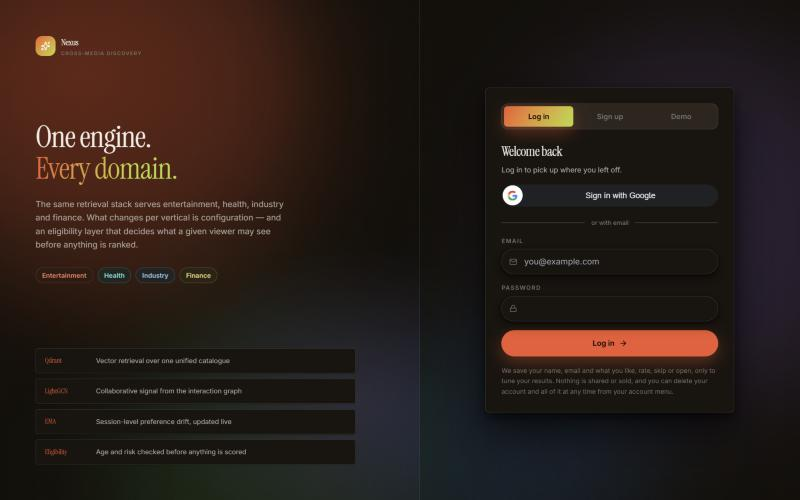
\includegraphics[width=\linewidth]{figures/login_page.jpg}\\[-1pt]
        {\scriptsize (a) Sign-in: email, Google or a demo profile, with a privacy notice}
    \end{minipage}\hspace{0.03\textwidth}
    \begin{minipage}{0.47\textwidth}\centering
        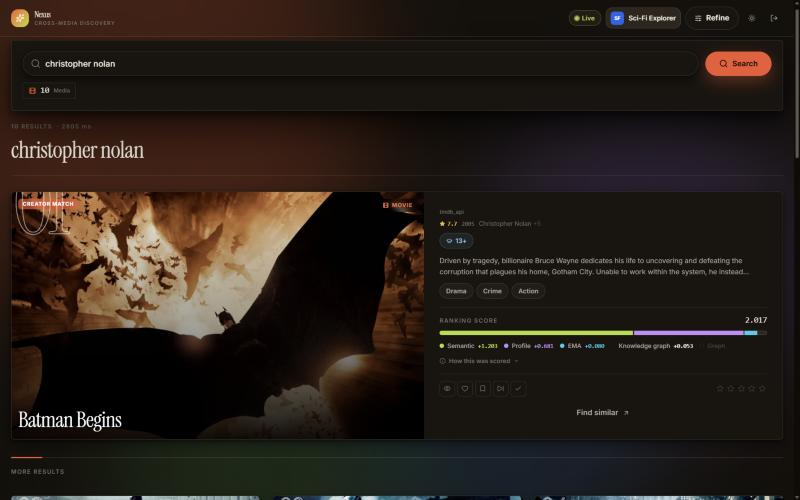
\includegraphics[width=\linewidth]{figures/search_results.jpg}\\[-1pt]
        {\scriptsize (b) Search ``christopher nolan'': creator match, score breakdown per signal}
    \end{minipage}\\[5pt]
    \begin{minipage}{0.47\textwidth}\centering
        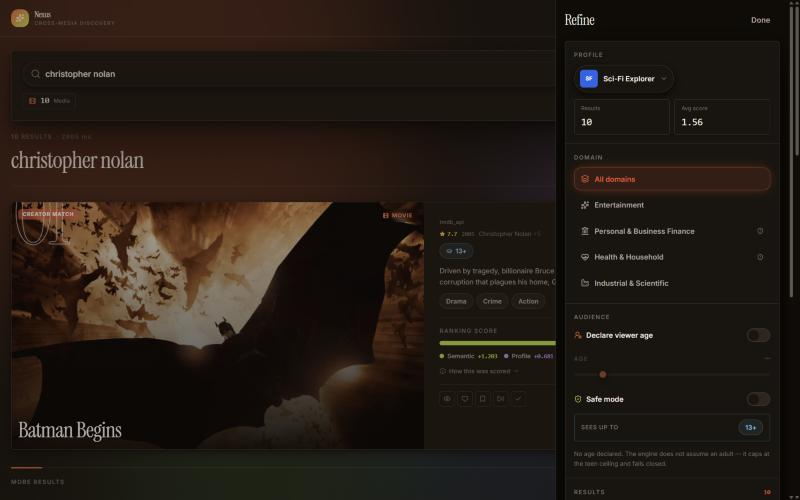
\includegraphics[width=\linewidth]{figures/refine_panel.jpg}\\[-1pt]
        {\scriptsize (c) Domain packs and audience controls; no age declared $\rightarrow$ teen ceiling}
    \end{minipage}\hspace{0.03\textwidth}
    \begin{minipage}{0.47\textwidth}\centering
        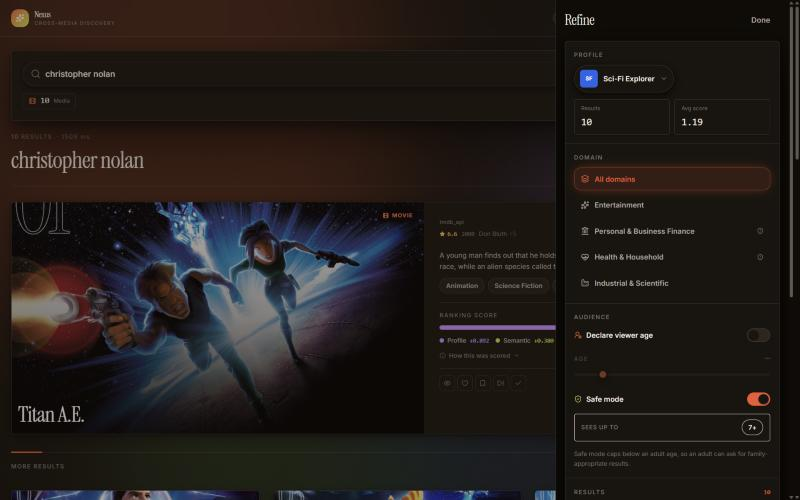
\includegraphics[width=\linewidth]{figures/safe_mode.jpg}\\[-1pt]
        {\scriptsize (d) Safe mode on: ceiling 7+, every 13+ Nolan film removed before scoring}
    \end{minipage}\\[5pt]
    \begin{minipage}{0.47\textwidth}\centering
        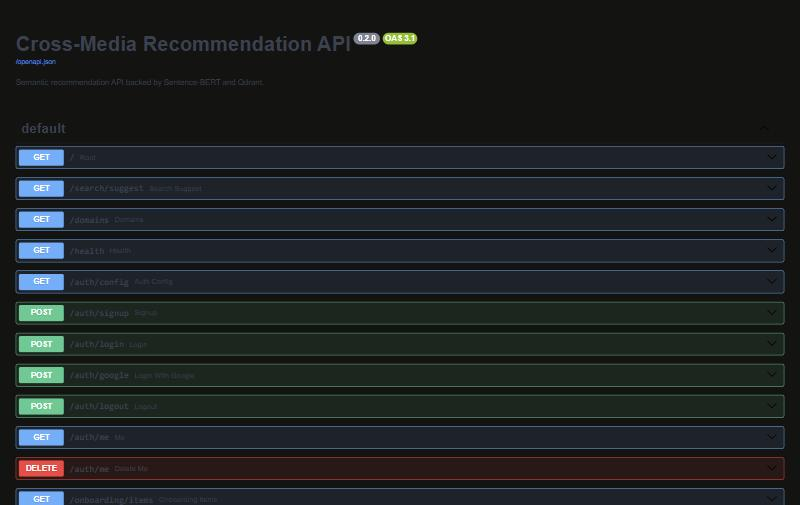
\includegraphics[width=\linewidth]{figures/swagger_api.jpg}\\[-1pt]
        {\scriptsize (e) The running API's interactive documentation (\texttt{/docs})}
    \end{minipage}
    \caption{Integrated Software System Demonstration and Test Execution Outputs (captured from the deployed build).}\label{fig:demo}
\end{figure}

% --- 6. TECHNICAL KNOWLEDGE & ENGINEERING DECISIONS ---
\section{Software Engineering Decisions \& Technical Justification}
\begin{itemize}[noitemsep, topsep=2pt]
    \item \textbf{Architectural \& Design Patterns:} A layered architecture with dependency injection (FastAPI \texttt{Depends}) keeps handlers testable with fakes; heavy models are singletons created in the application's \texttt{lifespan}. Domains are a configuration-driven registry, so a vertical is a YAML entry. The two-stage \emph{eligibility then relevance} design puts the safety rule where no reranker can override it. Additive late fusion was chosen over a learned black box because it lets the interface show each signal's exact contribution and supports counterfactual re-ranking.
    \item \textbf{Model choices:} SBERT MiniLM (384-d) encodes a query in about 13 ms, which keeps semantic search inside the latency budget. LightGCN stays in the serving path rather than NeuMF because its embeddings are precomputed and scored by a dot product (0.07 ms per request), sit beside the other vector signals, and propagate taste over the interaction graph; NeuMF needs a network evaluation per user--item pair. The dot-product result in Table~\ref{tab:cf} shows the remaining gain lies in how LightGCN is scored, not in replacing it.
    \item \textbf{Concurrency, Data Integrity \& Security:} Foreign keys cascade from the catalogue to the event log and from users to sessions; account deletion is one transaction; catalogue loads upsert in 2,000-row chunks and then prune stale rows. Pooled connections reset their session when returned, so no transaction or session state leaks between requests. Passwords are hashed with Argon2id; the session cookie is HttpOnly and SameSite=Lax and only its SHA-256 is stored; Google ID tokens are verified on the server; five wrong passwords lock an email for 15 minutes using the database clock; every request that names an account needs that account's session. All input is validated by Pydantic models.
    \item \textbf{Error Handling, Logging \& Maintainability:} Errors map to explicit status codes (400 invalid input, 401/403 access, 429 lockout, 503 dependency unavailable), and the API never falls back to an unfiltered search after an internal error. Unknown values fail closed. Server output is logged per run (\texttt{logs/}). The code is organised by layer (\texttt{backend/}, \texttt{preprocessing/}, \texttt{embeddings/}, \texttt{models/}, \texttt{scripts/}, \texttt{frontend/}), and 381 tests plus CI guard every change.
\end{itemize}

% --- 7. CONCLUSION, LIMITATIONS & FUTURE SCOPE ---
\section{Conclusion, Limitations \& Future Scope}
\begin{itemize}[noitemsep, topsep=2pt]
    \item \textbf{Conclusion:} The project delivers a working, integrated, multi-domain recommendation system: hybrid retrieval with eligibility enforced inside the vector query, real-time adaptation without retraining, explainable additive ranking, and a complete account system, deployed with one command and verified by 381 tests, a latency study, a zero-violation constraint evaluation and benchmarked collaborative models. Both recommendations of the previous review are addressed: age-based filtering is in production, and the NCF baseline is implemented and measured.
    \item \textbf{Known Limitations:} The system runs on a single machine with embedded Qdrant; there is no permanent host or container image yet. The knowledge-graph signal is term overlap, not graph traversal. The in-app LightGCN model is trained on the 13 seeded personas because the platform has no real user base; the benchmarks are the evidence for the model. LightGCN is served by cosine, which measurably under-ranks it. Fusion weights are hand-set, and the personalisation bonus can outweigh weak relevance for heavily profiled users. Book and music maturity labels are keyword heuristics. There is no email verification or password reset. The SBERT model is English-only and ignores negation.
    \item \textbf{Future Roadmap:} Serve LightGCN by a rescaled dot product; keep NeuMF as a pluggable collaborative signal and tune both with several seeds; replace term overlap with a typed knowledge graph (for example Neo4j) and path-based scoring; package the services with Docker and deploy Qdrant as a server with payload indexes; learn the fusion weights from real interaction logs; add a multilingual encoder, email verification and password reset.
\end{itemize}

% --- 8. DELIVERABLES & TECHNICAL ENRICHMENT SUMMARY ---
\section{Project Deliverables \& Technical Enrichment Summary}
\begin{table}[H]
    \centering
    \footnotesize
    \renewcommand{\arraystretch}{1.2}
    \begin{tabular}{|L{4.2cm}|L{9.4cm}|c|}
        \hline
        \textbf{Deliverable Category} & \textbf{Details / Title / Repository Link} & \textbf{Status} \\
        \hline
        Source Code Repository & \url{https://github.com/sanjay-pokee/Real-Time-Adaptive-Cross-Media-Recommendation-System}; README covers setup, API, evaluation and limitations; CI on every push. & Completed \\
        \hline
        Research Publication & ``Real-Time Adaptive Cross-Media Recommendation Using Semantic Embeddings, Knowledge Graph Scoring, and Graph Collaborative Learning'', ICMLDE 2026, Procedia Computer Science \cite{ak2026crossmedia}. & Accepted \\
        \hline
        Individual Online Certifications & Sanjay A. K.: Recommender Systems: Evaluation and Metrics (Coursera, Univ. of Minnesota, 15 h); Eswara Raj M.: Nearest Neighbor Collaborative Filtering (Coursera, Univ. of Minnesota, 14 h); Aditya Vijay: Databases and SQL for Data Science with Python (Coursera, IBM, 20 h); Himaneesh Reddy J.: Recommendation Systems on Google Cloud (Google Cloud Skills Boost, 16 h). & \fillin{confirm} \\
        \hline
        Group TEA Deliverable 1 & \fillin{Title and details of Group Activity 1} & \fillin{status} \\
        \hline
        Group TEA Deliverable 2 & \fillin{Title and details of Group Activity 2} & \fillin{status} \\
        \hline
        Group TEA Deliverable 3 & \fillin{Title and details of Group Activity 3} & \fillin{status} \\
        \hline
    \end{tabular}
    \caption{Summary of Completed Project and Technical Enrichment Deliverables}
\end{table}

% --- REFERENCES ---
\vspace{0.2cm}
\nocite{*}
\renewcommand{\refname}{\large\bfseries\color{amritaMaroon}References}
\bibliographystyle{ieeetr}
\bibliography{ref}

\end{document}
